\documentclass[t]{beamer}
\usetheme{Warsaw}
\usepackage{array}
\usepackage{graphicx}
\usepackage{amssymb,amsmath,mathrsfs,amsfonts}
%\usepackage[colorhighlight,display]{texpower}
%\usepackage{caption}
%\usepackage[all]{xy}
\usepackage{beamerthemesplit}
\mode<presentation>
%\usepackage{pause}
\usepackage{ulem}  % for strikethroughs
\usepackage{cancel} % for strikethroughs in math mode 
\usepackage{tikz}
\usepackage{calc}
\usetikzlibrary{shapes}
\usepackage{hyperref}
\hypersetup{pdfpagemode=FullScreen}
\usepackage{ifthen}
\usepackage{animate}
\usepackage{color}
\usepackage{type1cm}  % used for watermarking
\usepackage{eso-pic}  % used for watermarking


\theoremstyle{plain}
\newtheorem{prop}{Proposition}
\newtheorem{thm}[prop]{Theorem}
\newtheorem{lem}[prop]{Lemma}
\newtheorem{cor}[prop]{Corollary}
\theoremstyle{definition}
\newtheorem{dfn}{Definition}
\newtheorem{rem}[prop]{Remark}
\newtheorem{ex}{Example}[section]
%\newtheorem{note}{Note}[section]
\newtheorem{exercise}{Exercise}[section]
\newcommand{\nin}{\noindent}
\newcommand{\ds}{\displaystyle}
\renewcommand{\figurename}{Figure \arabic{figure}}



\renewcommand*\familydefault{\sfdefault} 




%%%%%%%%%%%%%%%%%%%%%%%%%%5
%%%%%%%%%%%%%%%%%%%%%%%%%%%%
%%%% some commands that have different meaning in the article/presentation modes

\newcommand{\vvfill}{\mode<presentation>{\vfill}  \mode<article>{\medskip}}   %vfill in presentation only
\newcommand{\sketchspace}{ 
\mode<article>{ \medskip\noindent{\textbf{Sketch:}} \vspace*{6cm} }
\mode<presentation>{ } 
}
\newcommand{\examplespace}{ 
\mode<article>{ \medskip\noindent{\textbf{Example:}} \vspace{6cm} }
\mode<presentation>{ } 
}
\newcommand{\artsmspace}{\mode<article>{\vspace*{2cm}} }  %small space in article mode
\newcommand{\artlargespace}{\mode<article>{\vspace*{6cm}} }  %large space in article mode

\newcommand{\dx}{\,dx}

\newcommand{\soln}{{\textbf{Solution: }}\,\,\,}
\newcommand{\disp}{\displaystyle}

\newcommand{\makedate}{\vvfill
\begin{picture}(10,10)  
\put(260,-20){\mbox{\tiny{\today}}}
\end{picture}
}

\newcommand{\pd}[2]{\dfrac{\partial#1}{\partial#2}}
\newcommand{\pD}[2]{\dfrac{\partial^2#1}{\partial#2^2}}
\newcommand{\pdd}[3]{\dfrac{\partial^2#1}{\partial#2 \partial#3}}


\normalem %stops the ulem package making all the emphs into underlines...
 
 
 
 \newcommand{\refandrev}[2]{
 \begin{small}
  \hspace{6cm}
  \begin{minipage}[r]{8cm}
  Stewart,    Chapter #1   \\
  Review:  \parbox[t]{6cm}{#2}
\end{minipage}
\end{small}
}



\newcounter{heading}
\setcounter{section}{1}
\setcounter{heading}{0}

\newcommand{\makeheading}[1]{\medskip\begin{large}\noindent\textbf{{#1}}\end{large}\smallskip}

%\newenvironment{head}[1]{\medskip\stepcounter{heading}\noindent\textbf{\hspace{0.2cm}{#1}.}}{}
\newcommand{\newhead}[1]{\medskip\stepcounter{heading}\noindent\textbf{\hspace{0.2cm}{#1}.}}


\newcommand{\pf}[1]{\noindent\textit{Proof.}\vspace*{#1 cm}}
\newcommand{\sol}[1]{\noindent\textit{Solution.}\vspace*{#1 cm}}
\newcommand{\further}[1]{\begin{small}\noindent\textit{Further reading: #1}\end{small}}
\newcommand{\exr}[1]{\begin{footnotesize}\noindent\textit{\textbf{Exercises:} Stewart #1}\end{footnotesize}}


% Sets of numbers
\newcommand{\C}{\mathbb{C}}
\newcommand{\RR}{\mathbb{R}}
\newcommand{\Z}{\mathbb{Z}}
\newcommand{\N}{\mathbb{N}}
\newcommand{\Q}{\mathbb{Q}}

% Partitions
\newcommand{\PP}{\mathcal{P}}

% Limits
\newcommand{\limm}[1]{\displaystyle \lim_{x\to #1}}

% Backslash
\newcommand{\bs}{\backslash}

% functions
\newcommand{\cosec}{\mathrm{cosec}}
\newcommand{\cosech}{\mathrm{cosech}}
\newcommand{\sech}{\mathrm{sech}}
\newcommand{\Li}{\mathrm{Li}}
\newcommand{\si}{\mathrm{Si}}
\newcommand{\erf}{\mathrm{erf}}

% Domain and Range
\newcommand{\Dom}{\mathrm{Dom}}
\newcommand{\Codom}{\mathrm{Codom}}
\newcommand{\Range}{\mathrm{Ran}}



\title{Week 10:  The logarithmic and exponential functions, exponential growth}
\date{October 9 -- October 12, 2012}

\begin{document}

\frame{\titlepage}

\setcounter{tocdepth}{2}
\frame{\tableofcontents

\begin{flushright}
\hyperlink{wed}{\beamergotobutton{Lecture 18}}\\

\hyperlink{thurs}{\beamergotobutton{Lecture 19}}
\end{flushright} 
}

\AtBeginSection[]
{
\begin{frame}<beamer> 
\tableofcontents[currentsection]  % show TOC and highlight current section
\end{frame}
}

\begin{frame}
\frametitle{Recall from last class}
\begin{itemize}[<+->]
\item Since $\ln$ and $\exp$ are inverses and $\ln(e^{r}) = r\ln(e) = r$, this means that $\exp(r) = e^{r}$.
\item We \emph{define} $e^{x} = \exp(x)$ for all  $x \in \mathbb{R}$.  Therefore,
\[ e^{x} = y \qquad \text{and} \qquad \ln y = x.\]
\item $e^{x+y} = e^{x}e^{y}$
\item $e^{x-y} = \frac{e^{x}}{e^{y}}$
\item $(e^{x})^{r} = e^{rx}.$
\end{itemize}
\end{frame}

\begin{frame}
\newhead{Examples}
Find the limit:
\begin{enumerate}[<+->]
\item[(i)] $\limm{\infty} \frac{e^{3x} - e^{-3x}}{e^{3x} + e^{-3x}}$.

\vspace*{.5cm}

\item[(ii)] $\limm{2^{+}}e^{3/(2-x)}$
\end{enumerate}
\end{frame}

\begin{frame}
\noindent What is the derivative of $e^{x}$?  We know it is differentiable because it is the inverse function of $\ln x$, which is differentiable with nonzero derivative.  Let's use implicit differentiation to answer this question:\pause

\vspace*{.4cm}
\noindent Let $y=e^x$. Then, $\ln y=x$. \pause Differentiating both sides,
\[ \frac{1}{y}\cdot\frac{dy}{dx}=1.\]\pause
Thus, $\dfrac{dy}{dx}=y=e^x$.\pause

\newhead{(Important) derivative} $\frac{d}{dx}e^{x} = e^{x}$.  Moreover, up to multiplication by a constant, this is the \emph{only} function which is its own derivative!!
\end{frame}

\begin{frame}
\newhead{Examples}
\begin{enumerate}[<+->]
\item[(i)] Differentiate the function given by $y = \sqrt{1 + xe^{-2x}}$.
\vspace*{.5cm}
\item[(ii)] Find an equation of the tangent line to the curve $y = e^{x}/x$ at the point $(1, e)$.
\vspace*{.5cm}
\item[(iii)] On what interval is the curve $y = xe^{3x}$ concave upward?
\end{enumerate}


\end{frame}

\begin{frame}
\noindent What about integration?  Well, because $e^{x}$ has a simple derivative, it also has a simple antiderivative!  Namely
\[ \int e^{x} \, dx = e^{x} + C.\]\pause

\newhead{Example}  Evaluate the integral \[ \int \frac{e^{1/x}}{x^{2}}\,dx. \]
\end{frame}

\section{General exponential and logarithmic functions}
\begin{frame}
\noindent Now, as promised, we will finally be able to define $a^{x}$, where $a$ is a positive real number and $x$ is \emph{any} real number!  First, we observe that if $r$ is rational, then
\[ a^{r} = (e^{\ln a})^{r} = e^{r \ln a}.\]\pause
However, the right side of the equation makes sense even if $r$ is not rational, because we have defined $e^{x}$ for \emph{all} real $x$.  So if $x$ is real, we make the following definition:\pause

\begin{dfn} If $a>0$ and $x \in \mathbb{R}$, then
\[ a^{x} = e^{x \ln a}.\]\end{dfn}\pause
When we first introduced the problem of defining arbitrary exponential functions, we asked the question, what is $2^{\sqrt{3}}$?  Now we can answer it!
\[ 2^{\sqrt{3}} = e^{\sqrt{3}\ln 2} \]\pause


%\vfill
\end{frame}

\begin{frame}

\noindent We call a function defined by $f(x) = a^{x}$ an \textbf{exponential function with base $a$}.  We can see that such a function is always positive because $e^{x}$ is always positive.\pause

\vspace*{.5cm}

\newhead{Example}
Solve for $x$:\begin{enumerate}
\item $2^{x-5} = 3$.
\end{enumerate}
\end{frame}

\begin{frame}
\noindent Armed with this definition of an arbitrary exponential function, we can improve one of the properties of $\ln x$.  We showed earlier that $\ln (a^{r}) = r\ln a$ when $r$ is \emph{rational}.  But now,
if $x$ is any \emph{real} number, we notice that
\[ \ln(a^{x}) = \ln(e^{x \ln a}) = x \ln a,\]
so the formula holds in fact for any \emph{real} number!  \pause

\vspace*{.1cm}

\noindent We list this, and a few other properties.  The book justifies a few of these properties more.  In the following, we assume that $x,y$ are real numbers and $a,b$ are strictly positive.
\begin{itemize}[<+->]
\item $\ln a^{x} = x\ln a$ for any real number $x$.
\item $a^{x+y} = a^{x}a^{y}.$
\item $a^{x-y} = a^{x}/a^{y}$.
\item $(a^{x})^{y} = a^{xy}$.
\item $(ab)^{x} = a^{x}b^{x}$.
\end{itemize}
\end{frame}

\begin{frame}
\noindent What do the graphs of arbitrary exponential functions look like?\pause

\vspace*{1cm}

\noindent Finally, we see that $\frac{d}{dx}(a^{x}) = a^{x}\ln a$:\pause

\vspace*{1cm}

\newhead{Examples}
\begin{enumerate}[<+->]
\item[(i)] Write $(\cos x)^{x}$ as a power of $e$.
\vspace*{.3cm}
\item[(ii)] Differentiate the function $h(t) = t^{3} - 3^{t}$.
\end{enumerate}
\end{frame}

\begin{frame}
\noindent How do we integrate a general exponential function? \pause Since
\[ \frac{d}{dx}(a^{x}) = a^{x} \ln a,\]
this implies that
\[ \int a^{x}\, dx = \frac{a^{x}}{\ln a} + C, \qquad a \neq 1.\]\pause

\newhead{Example} Calculate $\int_{0}^{5}3^{x}\, dx.$ 


\end{frame}

\begin{frame}
\noindent We can now state the \textbf{general power rule}, namely if $n$ is \emph{any} real number and $f$ is given by $f(x) = x^{n}$, then
\[ f'(x) = nx^{n-1}.\]\pause

\vspace*{.5cm}

\newhead{Example}
Differentiate $y = x^{e^{x}}.$
\end{frame}

\begin{frame}
\label{wed}
\newhead{General Logarithmic Functions} If $a$ is positive and not equal to one, then $a^{x}$ is one-to-one.  Hence it has an inverse, denoted by $\log_{a}$, which is called the \textbf{logarithmic function with base $a$}.  That is,
\[ \log_{a}x = y \iff a^{y} = x.\]\pause

\medskip

\noindent We see that $\log_{e}x = \ln x$, and that
\[ a^{\log_{a}x} = x \qquad \textrm{and} \qquad \log_{a}(a^{x}) = x.\]\pause

\medskip

\noindent How does the graphs of the general logarithm look like?
\end{frame}

\begin{frame}
\noindent It is easy to check the  following important \textbf{change of base formula}, relating general logarithms to the natural logarithm:  If $a > 0$, $a\neq 1$, then
\[ \log_{a}x = \frac{\ln x}{\ln a}.\]\pause


\vspace*{.2cm}
\noindent This implies that 
\[ \frac{d}{dx}(\log_{a}x) = \frac{1}{x\ln a}.\]\pause


\vspace*{1cm}

\newhead{Example} Calculate the derivative of the function given by $f(x) = \log_{10}(2 + \sin x).$

\end{frame}

\begin{frame}
\noindent We briefly derive a formula for the number $e$ as a limit.  You may be familiar with this definition of $e$ from high school.  \pause

\vfill

\noindent We record this as 
\[ e = \limm{0}(1+x)^{1/x} \qquad \textrm{or equivalently} \qquad e = \lim_{n\rightarrow \infty}\Big(1 + \frac{1}{n}\Big)^{n}.\]
\end{frame}

\begin{frame}
\newhead{True or False?}
\begin{itemize}[<+->]
\item[(i)] If $0 < a < b$, then $\ln a < \ln b$.
\vspace*{.5cm}
\item[(ii)] $\pi^{\sqrt{5}} = e^{\sqrt{5}\ln\pi}$.
\vspace*{.5cm}
\item[(iii)] You can always divide by $e^{x}$.
\vspace*{.5cm}
\item[(iv)] If $a>0$ and $b>0$ then $\ln(a+b) = \ln a + \ln b$.
\vspace*{.5cm}
\item[(v)] If $x >0$, then $(\ln x)^{6} = 6 \ln x$.
\vspace*{.5cm}
\item[(vi)] $\frac{d}{dx}(10^{x}) = x10^{x-1}$.
\vspace*{.5cm}
\item[(vii)] $ \frac{d}{dx}(\ln 10) = \frac{1}{10}$.
\vspace*{.5cm}
\item[(viii)] The inverse function of $y = e^{3x}$ is $y = \frac{1}{3}\ln x$.
\end{itemize}
\end{frame}

\subsection{Exponential growth and decay}

\begin{frame}
\newhead{Exponential growth and decay}

\noindent We come to one of the most important applications of exponential functions.  In many natural phenomena, quantities grow or decay at a rate proportional to their size. \pause If $y(t)$ is the value of such a quantity at time $t$ then
\[\frac{dy}{dt}=ky,\]
where $k$ is the constant of proportionality.\pause

\vfill

\begin{theorem}
The only solutions of the differential equation $\dfrac{dy}{dt} = ky$ are the exponential functions \[ y(t) = y(0)e^{kt}.\]
\end{theorem}
\end{frame}

\begin{frame}
\newhead{Example: Population growth} The CIA World Fact Book estimated that the population of Australia in July 2009 was 21,262,641 and that its 2009 growth rate was 1.195\%. Estimate the population of Australia in July 2015, assuming that its growth rate remains constant.\pause

\vfill

\newhead{Remark} In population studies, the constant of proportionality $k$ is often called the \textit{(relative) growth rate}.

\end{frame}

\begin{frame}
\newhead{Radioactive decay} Radioactive substances decay by spontaneously emitting radiation. If $m(t)$ is the mass remaining from an initial mass $m_0$ then the relative decay rate has been found experimentally to be constant.\pause This means that
\[\frac{dm}{dt}=km\]
where $k<0$. The positive number $-k$ is called the decay rate.\pause

The {\em half-life} of a radioactive substance is the time required for half of any given quantity to decay.
\end{frame}

\begin{frame}

\newhead{Some Half-Lives}

\begin{tabular}{|c|c|c|}
  \hline
  % after \\: \hline or \cline{col1-col2} \cline{col3-col4} ...
  \textbf{Yield} & \textbf{Fission Product} & \textbf{Half-life}\\
  6.8\% & Cesium-134 & 2 years \\
  6.3\% & Iodine-135 & 7 hours \\
  6.1\% & Zirconium-93 & 1.5M years \\
  6.1\% & Cesium-137 & 30 years \\
  5.8\% & Technetium-99 & 200k years \\
  2.8\% & Iodine-131 & 8 days \\
  \hline
\end{tabular}\pause

\newhead{Example: Carbon dating}
Carbon-14 has a half-life of about 5730 years.
\begin{enumerate}[<+->]
\item[(a)] Suppose that $m(t)$ denotes the mass of Carbon-14 present in a fossil at time $t$. Find a formula for $m(t)$.
\item[(b)] The proportion of Carbon-14 in an animal fossil is 0.6\%.\\ Assume that when the animal died the proportion was 1\%.\\ Use this information to estimate when the animal died.
\end{enumerate}
\end{frame}

\begin{frame}
\newhead{Compound interest} Suppose that an amount $A_0$ is invested at an interest rate of $r$ per annum and is compounded $n$ times a year. Then the investment $A(t)$ in $t$ years is given by
\[A(t)=A_0\left(1+\frac{r}{n}\right)^{nt}.\]\pause

\noindent\textit{Example.} If $A_0=\$1000$ and $r=6\%$ per annum then the\\ investment in 3 years is worth:\pause
\begin{footnotesize}
\begin{align*}
\$1000(1.06)^3&=\$1191.02 \mbox{ with annual compounding ($n=1$)} \\
\$1000(1.03)^6&=\$1194.05  \mbox{ with half-yearly compounding ($n=2$)} \\
\$1000(1.015)^{12}&=\$1195.62  \mbox{ with quarterly compounding ($n=4$)} \\
\$1000(1.005)^{36}&=\$1196.68  \mbox{ with monthly compounding ($n=12$)} \\
\$1000\left(1+\frac{0.06}{365}\right)^{1095}&=\$1197.20  \mbox{ with daily compounding ($n=365$)}.
\end{align*}
\end{footnotesize}\pause

\noindent If we let $n\to\infty$, we will be compounding the interest \textit{continuously}.

\

\end{frame}

\begin{frame}
\noindent We derive a formula for continuous compounding:\pause

\medskip

\noindent We return now to the example of \$1000 invested at an interest rate of 6\% per annum. If the interest is compounded continuously then the amount after three years will be
\[A(3)=\$1000e^{(0.06)3}=\$1197.22.\]\pause
Notice how close this is to the amount for daily compounding. \\However, the formula using continuous compounding is much easier to manipulate mathematically.
\end{frame}

\section{Inverse  functions}
\subsection{The inverse trigonometric functions}

\begin{frame}
\frametitle{The inverse trig functions}


\noindent We now leave behind $\ln x$ and $e^{x}$ and examine inverse functions to another familiar class of examples, the trigonometric functions.  Consider the graph of $\sin x$:\pause

\begin{center}
\begin{tikzpicture}[scale=0.6]
\draw[loosely dotted]  (-4,-2) grid (4,2);
\draw[blue, thick, domain=-pi:3.6] plot[id=sin] function{sin(x)} node[right] {$y=\sin(x)$};
\draw[->] (-4.2,0) -- (4.2,0) node[right] {$x$};
\draw[->] (0,-2.25) -- (0,2.25) node[above] {$y$};
\foreach \x/\xtext in {pi/{\pi}, -pi/{-\pi}, {pi/2}/{\frac{\pi}{2}}, {-pi/2}/{-\frac{\pi}{2}}}
    \draw[shift={(\x,0)}] (0pt,2pt) -- (0pt,-2pt) node[below] {$\xtext$};
\foreach \y/\ytext in {1/1, 2/2,  -1/{-1}, -2/{-2}}
    \draw[shift={(0,\y)}] (2pt,0pt) -- (-2pt,0pt) node[left] {$\ytext$};
\end{tikzpicture}
\end{center}\pause

%\vspace*{2cm}
\noindent Notice that this is not one-to-one, but if we restrict $x$ to lie in $[\frac{-\pi}{2}, \frac{\pi}{2}]$, then $\sin x$ \emph{is} one-to-one, hence it has an inverse.  We denote this inverse by $\sin^{-1} x$.  
\end{frame}

\begin{frame}
Note that $\sin^{-1}x$ is \textbf{NOT} equal to $\frac{1}{\sin x}$.  Here is the graph of $\sin^{-1}x$:\pause

\begin{center}
\begin{tikzpicture}[scale=0.8]
\draw[loosely dotted, step=.5]  (-1,-1.5) grid (1,1.5);
\draw[blue, thick, domain=-1:1] plot[id=sin1] function{asin(x)} node[right] {$y=\sin^{-1}(x)$};
\draw[->] (-1.2,0) -- (1.2,0) node[right] {$x$};
\draw[->] (0,-1.75) -- (0,1.75) node[above] {$y$};
\foreach \x/\xtext in {1/1, 0/0,  -1/{-1}}
    \draw[shift={(\x,0)}] (0pt,2pt) -- (0pt,-2pt) node[below] {$\xtext$};
\foreach \y/\ytext in {1/1, {pi/2}/{\frac{\pi}{2}}, {-pi/2}/{-\frac{\pi}{2}},  -1/{-1}}
    \draw[shift={(0,\y)}] (2pt,0pt) -- (-2pt,0pt) node[left] {$\ytext$};
\end{tikzpicture}
\end{center}\pause

\noindent We have
\[ \sin^{-1}x = y \iff \sin y = x \qquad \text{and} \qquad \frac{-\pi}{2} \leq y \leq \frac{\pi}{2}.\]\pause
That is, if $x \in [-1, 1]$, then $\sin^{-1}x$ is the number between $\frac{-\pi}{2}$ and $\frac{\pi}{2}$ whose sine is $x$.  The domain of $\sin^{-1}x$ is $[-1,1]$ and the range is $[-\frac{\pi}{2}, \frac{\pi}{2}]$.
\end{frame}

\begin{frame}\label{thurs}
\noindent The cancellation formulas for $\sin^{-1}$ are:
\begin{align*}
\sin^{-1}(\sin x) &= x \qquad \text{for } \frac{-\pi}{2} \leq x \leq \frac{\pi}{2}\\
\sin(\sin^{-1}x) &= x \qquad \text{for } -1 \leq x \leq 1.
\end{align*}\pause

\medskip

\noindent Let's use implicit differentiation to calculate the derivative of $\sin^{-1}$:\pause

\noindent Therefore we have
\[ \frac{d}{dx}(\sin^{-1}x) = \frac{1}{\sqrt{1-x^{2}}},\qquad -1 < x < 1.\]\pause

\newhead{Example} If $f(x) = \sin^{-1}(x^{2} - 1)$, find (a) the domain of $f$, (b) the derivative $f'(x)$, and (c) the domain of $f'$.
\end{frame}

\begin{frame}
\noindent What about $\cos^{-1}$? Here is the graph of $y = \cos x$:\pause


\begin{center}
\begin{tikzpicture}[scale=0.6]
\draw[loosely dotted]  (-4,-2) grid (4,2);
\draw[blue, thick, domain=-pi:3.6] plot[id=cos] function{cos(x)} node[right] {$y=\cos(x)$};
\draw[->] (-4.2,0) -- (4.2,0) node[right] {$x$};
\draw[->] (0,-2.25) -- (0,2.25) node[above] {$y$};
\foreach \x/\xtext in {pi/{\pi}, -pi/{-\pi}, {pi/2}/{\frac{\pi}{2}}, {-pi/2}/{-\frac{\pi}{2}}}
    \draw[shift={(\x,0)}] (0pt,2pt) -- (0pt,-2pt) node[below] {$\xtext$};
\foreach \y/\ytext in {1/1, 2/2,  -1/{-1}, -2/{-2}}
    \draw[shift={(0,\y)}] (2pt,0pt) -- (-2pt,0pt) node[left] {$\ytext$};
\end{tikzpicture}
\end{center}\pause

\noindent We must again restrict the domain of $\cos x$ so that it is one-to-one.  We restrict $x$ to lie in $[0,\pi]$, then define the inverse function, denoted by $\cos^{-1}x$.  
\end{frame}

\begin{frame}
Its graph looks like this:

\begin{center}
\begin{tikzpicture}[scale=0.6]
\draw[loosely dotted, step=.5]  (-1,0) grid (1,3.5);
\draw[blue, thick, domain=-1:1] plot[id=cos1] function{acos(x)} node[above right] {$y=\cos^{-1}(x)$};
\draw[->] (-1.2,0) -- (1.2,0) node[right] {$x$};
\draw[->] (0,-.25) -- (0,3.56) node[above] {$y$};
\foreach \x/\xtext in {1/1, 0/0,  -1/{-1}}
    \draw[shift={(\x,0)}] (0pt,2pt) -- (0pt,-2pt) node[below] {$\xtext$};
\foreach \y/\ytext in {1/1, {pi/2}/{\frac{\pi}{2}}, pi/{\pi}}
    \draw[shift={(0,\y)}] (2pt,0pt) -- (-2pt,0pt) node[left] {$\ytext$};
\end{tikzpicture}
\end{center}\pause
We summarize properties of $\cos^{-1}$:
\begin{itemize}[<+->]
\item $\cos^{-1}x$ has domain $[-1, 1]$ and range $[0,\pi]$.
\item $\cos^{-1}x = y \iff \cos y = x \qquad \textrm{and} \qquad 0 \leq y \leq \pi$.
\item $\cos^{-1}(\cos x) = x \qquad \textrm{for } 0 \leq x \leq \pi.$
\item $\cos(\cos^{-1} x) = x \qquad \textrm{for } -1 \leq x \leq 1.$
\item $\frac{d}{dx}(\cos^{-1}x) = - \frac{1}{\sqrt{1-x^{2}}} \qquad -1 < x < 1$.
\end{itemize}
\end{frame}

\begin{frame}
\noindent What about $\tan^{-1}$?  Here is the graph of $y = \tan x$, where we restrict $x$ to lie in $(-\frac{\pi}{2}, \frac{\pi}{2})$:\pause

\begin{center}
\begin{tikzpicture}[scale=0.36]
\draw[loosely dotted]  (-2,-8) grid (2,8);
\draw[blue, thick, domain=-1.45:1.45] plot[id=tan] function{tan(x)} node[right] {$y=\tan(x)$};
\draw[->] (-2.1,0) -- (2.1,0) node[right] {$x$};
\draw[->] (0,-8.25) -- (0,8.25) node[above] {$y$};
\foreach \x/\xtext in {{pi/2}/{\frac{\pi}{2}}, {-pi/2}/{-\frac{\pi}{2}}}
    \draw[shift={(\x,0)}] (0pt,2pt) -- (0pt,-2pt) node[below] {$\xtext$};
\foreach \y/\ytext in {6/6, 2/2,  -6/{-6}, -2/{-2}, 4/4, -4/{-4}, 8/8, -8/{-8}}
    \draw[shift={(0,\y)}] (2pt,0pt) -- (-2pt,0pt) node[left] {$\ytext$};
\draw[blue, thin,  dashed] (pi/2,-7.9) -- (pi/2,7.9);
\draw[blue, thin,  dashed] (-pi/2,-7.9) -- (-pi/2,7.9);
\end{tikzpicture}
\end{center}

\end{frame}

\begin{frame}
\noindent With $x$ restricted in this way, $\tan x$ is one-to-one, hence it has an inverse function, denoted by $\tan^{-1}$. \pause The graph of $\tan^{-1}$ looks like this:

\begin{center}
\begin{tikzpicture}[scale=0.6]
\draw[loosely dotted]  (-8,-2) grid (8,2);
\draw[blue, thick, domain=-8:8] plot[id=tan1] function{atan(x)} node[above] {$y=\tan^{-1}(x)$};
\draw[->] (-8.2,0) -- (8.2,0) node[right] {$x$};
\draw[->] (0,-2.15) -- (0,2.15) node[above] {$y$};
\foreach \x/\xtext in {6/6, 2/2,  -6/{-6}, -2/{-2}, 4/4, -4/{-4}, 8/8, -8/{-8}}
    \draw[shift={(\x,0)}] (0pt,2pt) -- (0pt,-2pt) node[below] {$\xtext$};
\foreach \y/\ytext in {1/1, {pi/2}/{\frac{\pi}{2}}, {-pi/2}/{-\frac{\pi}{2}},  -1/{-1}}
    \draw[shift={(0,\y)}] (2pt,0pt) -- (-2pt,0pt) node[left] {$\ytext$};
\end{tikzpicture}
\end{center}\pause

We summarize some properties of $\tan^{-1}$:
\begin{itemize}[<+->]
\item $\tan^{-1}x = y \iff \tan y = x \qquad \text{and } -\frac{\pi}{2} < y < \frac{\pi}{2}$.
\item $\limm{\infty}\tan^{-1}x = \frac{\pi}{2} \qquad \limm{-\infty} \tan^{-1}x = -\frac{\pi}{2}.$
\item $\frac{d}{dx}(\tan^{-1}x) = \frac{1}{1 + x^{2}}.$
\end{itemize}
\end{frame}

\begin{frame}
\newhead{Remarks} Note that $\sin^{-1}x$, $\cos^{-1}x$, $\tan^{-1}x$, etc are often also called $\arcsin$, $\arccos$, $\arctan$, etc.  Also, note that one can discuss the definition and basic properties (such as derivatives) of the inverse functions to $\sec$, $\csc$, and $\cot$.  \pause

\vspace*{.5cm}
\newhead{Example} Simplify the expression $\cos(\tan^{-1}x)$.\pause

\vspace*{.3cm}
\newhead{Example} Differentiate the function given by $f(x) = x\tan^{-1}\sqrt{x}$.
\end{frame}

\subsection{The hyperbolic functions}

\begin{frame}
\frametitle{The hyperbolic functions}

\uncover<+->{\noindent There is another important and useful class of functions we will briefly study, known as the \textbf{hyperbolic functions}.  They are similar to trigonometric functions, but are closely related to the hyperbola instead of to the circle.  Here are the definitions:}

\begin{itemize}[<+->]
\item $\sinh x = \frac{e^{x} - e^{-x}}{2}.$
\item $\cosh x = \frac{e^{x} + e^{-x}}{2}.$
\item $\tanh x = \frac{\sinh x}{\cosh x}.$
\item $\text{csch } x = \frac{1}{\sinh x}.$
\item $\text{sech } x = \frac{1}{\cosh x}.$
\item $\coth x = \frac{\cosh x}{\sinh x}.$
\end{itemize}
\end{frame}

\begin{frame}
We draw the graphs of $\sinh$, $\cosh$, and $\tanh$:

\begin{center}
\begin{columns}[t]
\begin{column}{0.5\textwidth}
\begin{figure}
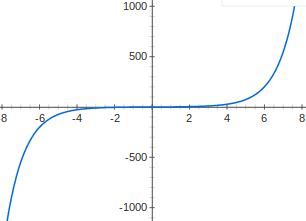
\includegraphics[scale=.3]{sinhx.png}
\caption{$y=\sinh x$}
\end{figure}
\end{column}
\begin{column}{0.5\textwidth}
\begin{figure}
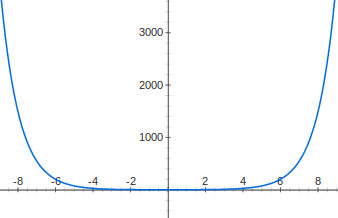
\includegraphics[scale=.3]{coshx.png}
\caption{$y=\cosh x$}
\end{figure}
\end{column}
\end{columns}
\begin{figure}
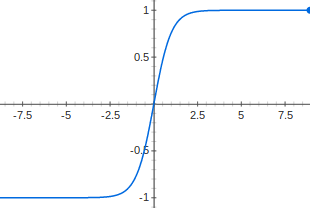
\includegraphics[scale=.3]{tanhx.png}
\caption{$y=\tanh x$}
\end{figure}
\end{center}
\end{frame}

\begin{frame}
\uncover<+->{\newhead{Properties of $\cosh$ and $\sinh$}  Notice how similar the following properties are to those of the trigonometric functions:}
\begin{itemize}[<+->]
\item $\sinh(-x) = -\sinh x$.
\item $\cosh(-x) = \cosh x$.
\item $\cosh^{2}x - \sinh^{2}x = 1.$
\item $1 - \tanh^{2}x = \text{sech}^{2}x.$
\end{itemize}
\uncover<+->{We prove the third property in the above list:}
\vspace*{.3cm}

\uncover<+->{\noindent We now can get some insight into why these functions are called ``hyperbolic''.  Notice that if $t$ is a real number, then the point $(\cosh t, \sinh t)$ lies on the right branch of the hyperbola $x^{2} - y^{2} = 1$.  It lies on the right branch because $\cosh t \geq 1$:}
\end{frame}

\begin{frame}
\noindent We now list formulas for the derivatives of the hyperbolic functions.  Note the similarities to the derivatives of the trigonometric functions (and the differences!):
\begin{itemize}[<+->]
\item $\frac{d}{dx}(\sinh x) = \cosh x$.
\item $\frac{d}{dx}(\cosh x) = \sinh x$.
\item $\frac{d}{dx}(\tanh x) = \text{sech}^{2}x$.
\item $\frac{d}{dx}(\text{csch }x) = - \text{csch }x\coth x$.
\item $\frac{d}{dx}(\text{sech }x) = - \text{sech }x\tanh x$.
\item $\frac{d}{dx}(\coth x) = - \text{csch }^{2}x$.
\end{itemize}

\medskip

\uncover<+->{\newhead{Example} Find the derivative: $y = e^{\cosh 3x}$.}
\end{frame}

\begin{frame}
\newhead{Example} If $\tanh x = \frac{4}{5}$, find the values of the other hyperbolic functions at $x$.\pause


\vfill
\newhead{Remark} In the textbook there are similar formulas for the inverse hyperbolic functions and their derivatives.  Although you will have webassign questions and a tutorial quiz on the hyperbolic functions and their inverses, I will not emphasize them on the final exam to the same extent as the trigonometric functions and their inverses.  \textbf{That is, you are expected to be familiar with hyperbolic functions and their inverses.  I may ask you questions involving these functions on the final exam, but if I do, they will be very basic questions.}
\end{frame}

\begin{frame}
\frametitle{Indeterminate Forms and L'Hospital's Rule}

\uncover<+->{\noindent Earlier in the semester we discussed limits of the form $\frac{\infty}{\infty}$. Such limits could be}
\begin{enumerate}[<+->]
\item[(a)] zero, e.g. $\ds \lim_{x\to\infty}\frac{2x}{x^2+1}=0$;
\item[(b)] infinite, e.g. $\ds \lim_{x\to\infty}\frac{x^2+6}{x}=\infty$;
\item[(c)] or somewhere between, e.g. $\ds \lim_{x\to\infty}\frac{3x^2+6}{x^2-x}=3$.
\end{enumerate}
\uncover<+->{Because one cannot say in advance exactly what a limit of the form $\frac{\infty}{\infty}$ will be, we call it an \textit{indeterminate form}.} \uncover<+->{Other indeterminate forms include
\[0\cdot\infty,\qquad \tfrac{0}{0}, \qquad\infty-\infty, \qquad0^0, \qquad \infty^0 \qquad\mbox{and}\qquad 0^{\infty}. \]}
\end{frame}

\begin{frame}
\uncover<+->{\noindent Each of the above limits (a), (b) and (c) can be calculated using the standard trick of dividing the denominator through by the fastest growing term. It is easy to tell which terms grow fastest because we are working with polynomials. What if this is not the case?} \uncover<+->{What about the following limits?
\[\lim_{x\to\infty}\frac{e^x}{x} \qquad\qquad\qquad \lim_{x\to\infty}\frac{\ln x}{x}\]}
\uncover<+->{In each case, does the denominator win out, or the numerator, or is there some kind of compromise?}
\end{frame}

\begin{frame}
\uncover<+->{\noindent One way to solve this problem is to look at the derivatives. \\}\uncover<+->{If, for example we could verify that
\[\lim_{x\to\infty}\frac{f'(x)}{g'(x)}=0\]
then this would suggest that the \textit{rate} of increase of $g$ is greater than that of $f$.}
\uncover<+->{ This in turn would suggest that
\[\lim_{x\to\infty}\frac{f(x)}{g(x)}=0.\]
In fact, this kind of intuitive reasoning is generally true!}
\end{frame}

\begin{frame}
\begin{block}{L'H\^opital's rule}
Suppose that $f$ and $g$ are differentiable functions, $a \in \mathbb{R}$, and $g'(x) \neq 0$, except possibly at $a$. Suppose also that either one of the two following conditions hold:
\begin{itemize}[<+->]
\item $f(x)\to0$ and $g(x)\to0$ as $x\to a$;
\item $f(x)\to\pm\infty$ and $g(x)\to\pm\infty$ as $x\to a$.
\end{itemize}
\uncover<+->{If
\[\limm{a}\frac{f'(x)}{g'(x)}\]
exists or is $\pm \infty$, then
\[\limm{a}\frac{f(x)}{g(x)}=\limm{a}\frac{f'(x)}{g'(x)}.\]}
\end{block}


\end{frame}


\end{document}